\section{Triangle-Feed Antenna}
\label{sec:triang_proto}
A prototype of the triangle-feed antenna has been built. The results will be described in this section.

The prototype is shown in Figure~\ref{fig:triang_proto}. Compared to the simulation, see Figure~\ref{fig:ant2techschem}, a \SI{5}{mm} strip of copper has been added next to the feed line. A free-space simulation has been made with the added copper strip for comparison.

\begin{figure}[htbp]
    \centering
    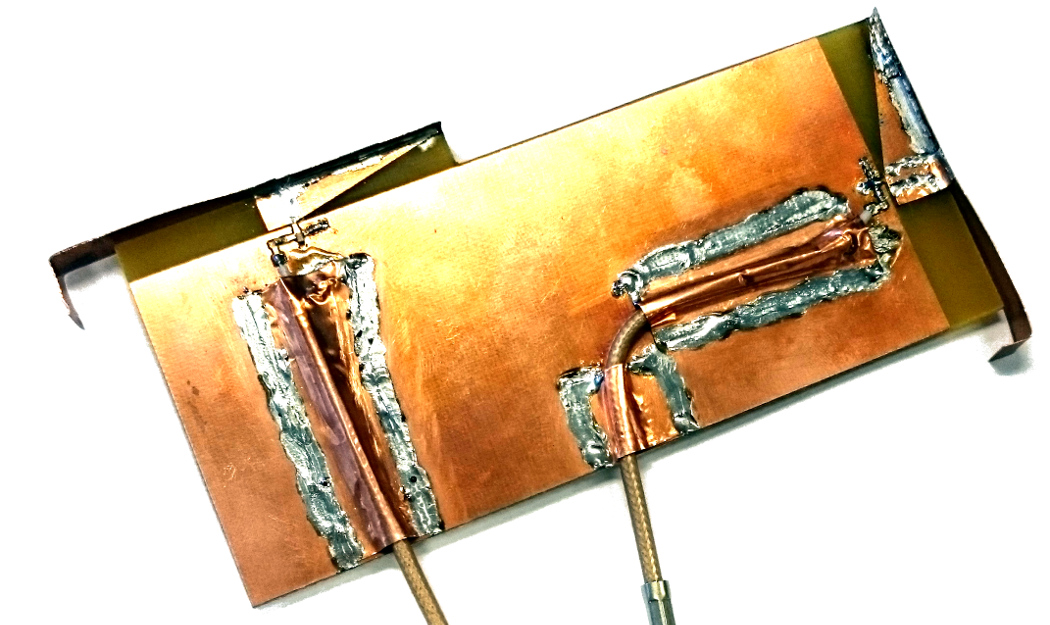
\includegraphics{img/tech_sol/trianglefeed/mockup/mockup.jpg}
    \caption{Triangle-feed antenna prototype.}
    \label{fig:triang_proto}
\end{figure}

\subsection{Measurement and Simulation Comparison}
The measured and simulated S-parameters and total efficiency is shown in Figure~\ref{fig:triang_proto_sparam_eff}. The component values used in the measurement are shown in Figure~\ref{fig:triang_proto_matching}. From the S-parameters it is seen that, in general, the resonances of the measurement correspond well with the resonances of the simulation -- especially for the top antenna. The levels of the return loss peaks are not the same but the antenna is nearly compliant with the impedance bandwidth requirement at \SI{5}{dB} return loss. The isolation is better than the simulated, peaking at around \SI{-8}{dB}. The efficiency is generally slightly lower than the simulated. This is to be expected as real-life matching components are lossy due to their Equivalent Series Resistance (ESR). It is seen that the efficiency bandwidth of the side antenna in the low band is greater than the simulation. This is due to the more wide-band matching seen in the corresponding S-parameters, S22, in the low band. Generally, the efficiency peaks correspond well with the return loss peaks and is quite good, peaking at above \SI{-3}{dB} in both the high and the low band.

The highest achievable bandwidth for both antennas, can be seen in Table \ref{tab:bw_sol2_proto}. From the table it is seen, that both antennas covers the required bandwidth quite well except for the top antenna. The top antenna is experiencing some problems in the high band, as it only covers \SI{500}{MHz}. This however does not seem like a big problem, as the bandwidth taken at \SI{-5}{dB} covers approximately \SI{1000}{MHz}.

\begin{figure}[htbp]
        \centering
        \begin{tabular}{m{3in}m{3in}}
            \centering
            \includegraphics{img/tech_sol/schematic_tuning_1}&
            \centering
            \footnotesize
            \begin{tabular}{|l|l|l|l|}
                \hline
                & $C_1$ & $L_1$ & $C_2$ \\
                \hline
                Top antenna & \SI{3.0}{pF} & \SI{6.8}{nH} & \SI{0.9}{pF} \\
                Side antenna & \SI{2.2}{pF} & \SI{5.6}{nH} & \SI{0.3}{pF} \\
                \hline
            \end{tabular}
        \end{tabular}
    \caption{Matching circuit for the triangle-feed antenna prototype. These are the component values where the bandwidth is found to be the largest.}
    \label{fig:triang_proto_matching}
\end{figure}

 \begin{figure}[htbp]
    \centering
    \begin{subfigure}{0.49\linewidth}
        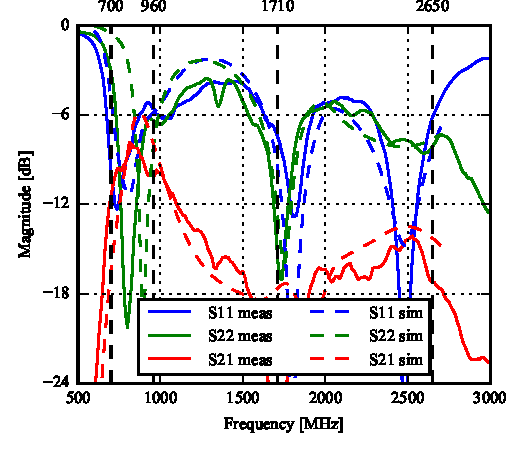
\includegraphics{img/tech_sol/trianglefeed/mockup/best_sparams.pdf}
        \caption{S-parameters.}
    \end{subfigure}
    \hfill
    \begin{subfigure}{0.49\linewidth}
        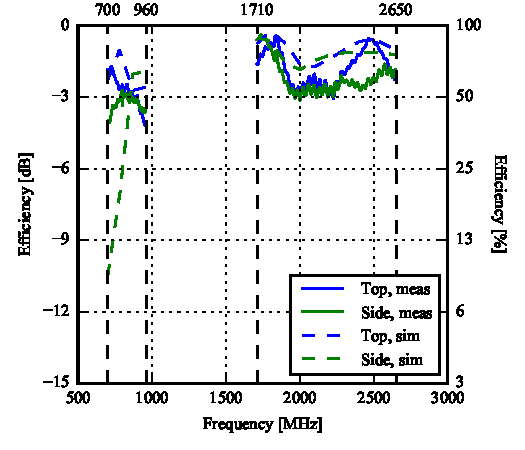
\includegraphics{img/tech_sol/trianglefeed/mockup/best_efficiency.pdf}
        \caption{Total efficiency.}
    \end{subfigure}
    \caption{S-parameters and total efficiency of the triangle-feed antenna prototype with the component values from Figure~\ref{fig:triang_proto_matching}.}
    \label{fig:triang_proto_sparam_eff}
\end{figure}

   \begin{table}
      \centering
      \begin{tabular}{|l|l|r|r|r|}
        \hline
        Antenna & Band & Start [MHz] & Stop [MHz] & Bandwidth [MHz] \\
        \hline
        Top     & Low  & 690        & 870       & 180 \\
        Side    & Low  & 710         & 1050        & 340 \\
        \hline
        Top     & High & 2250        & 2750       & 500 \\
        Side    & High & 2280        & 3000       & 720 \\
        \hline
      \end{tabular}
      \caption{Maximum bandwidth obtained in the low and high band for the top and the side antenna, respectively.}
      \label{tab:bw_sol2_proto}
    \end{table}

In addition to the S-parameters and the total efficiency, the envelope correlation coefficient has also been computed for the prototype. The result is shown in Figure~\ref{fig:triang_proto_ecc}, compared to the simulation. It is clearly seen that the simulated and measured correlation coefficients are very different. The reason for this is, most likely, that the antenna was not perfectly aligned when the top antenna and the side antenna were measured. To obtain realistic correlation results, the antenna should be located in the \emph{exact} same position for every measurement.

\begin{figure}[htbp]
    \centering
    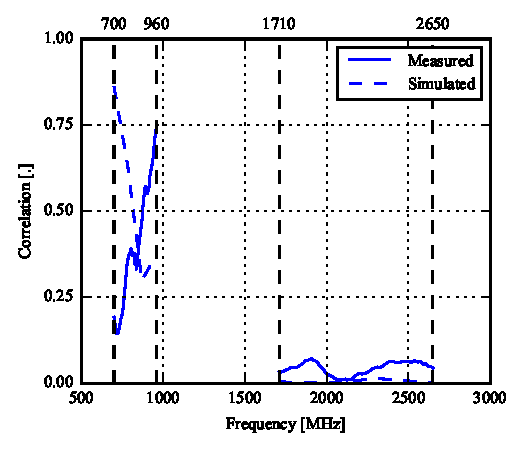
\includegraphics{img/tech_sol/trianglefeed/mockup/best_correlation.pdf}
    \caption{Measured and simulated envelope correlation coefficient for the triangle-feed antenna.}
    \label{fig:triang_proto_ecc}
\end{figure}

\subsection{Capacitor Sweep}
The shunt capacitor for each antenna has been swept to see the tuning ranges of the antennas. The S-parameters are shown in Figure~\ref{fig:triang_proto_sweep_sparams}. The efficiency-sweeps are shown in Figure~\ref{fig:triang_proto_sweep_efficiency}. All component values, except the shunt capacitors, are the same values as in Figure~\ref{fig:triang_proto_matching}.

From the S-parameters, it is seen that both the high and the low band for both antennas are covered at a return loss greater than \SI{5}{dB} for the low capacitance settings. Both antennas can be tuned down using the shunt capacitor to cover the lower part of the low band.

From the total efficiency, the same trend is seen. The efficiency can, generally, be tuned to be above \SI{-3}{dB} for both antennas in both the low and the high band.

\begin{figure}[htbp]
    \centering
    \begin{subfigure}{0.49\linewidth}
        \centering
        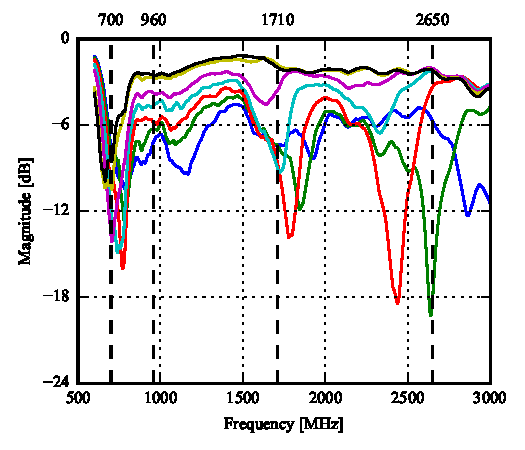
\includegraphics{img/tech_sol/trianglefeed/mockup/sweep_s11_csh1.pdf}
        \caption{$S_{11}$, sweeping the top antenna and fixing the side antenna.}
    \end{subfigure}
    \hfill
    \begin{subfigure}{0.49\linewidth}
        \centering
        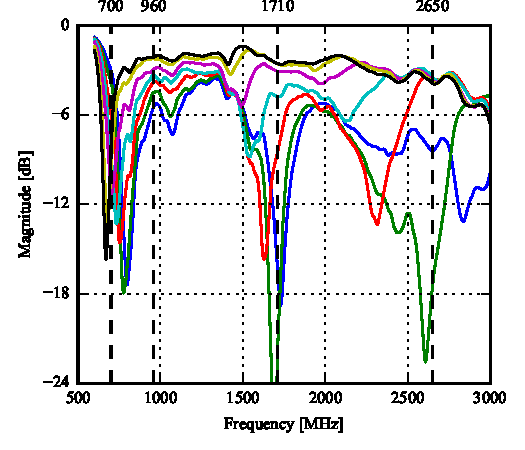
\includegraphics{img/tech_sol/trianglefeed/mockup/sweep_s22_csh2.pdf}
        \caption{$S_{22}$, sweeping the side antenna and fixing the top antenna.}
    \end{subfigure}
    \\
    \begin{subfigure}{0.49\linewidth}
        \centering
        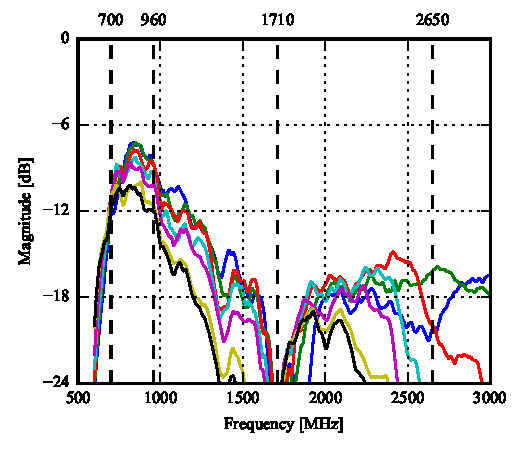
\includegraphics{img/tech_sol/trianglefeed/mockup/sweep_s21_csh1.pdf}
        \caption{$S_{21}$, sweeping the top antenna and fixing the side antenna.}
    \end{subfigure}
    \hfill
    \begin{subfigure}{0.49\linewidth}
        \centering
        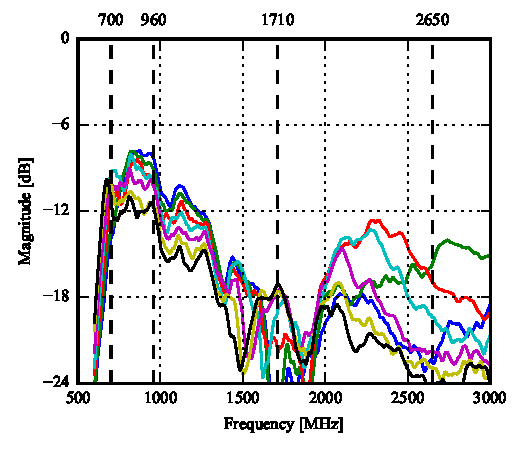
\includegraphics{img/tech_sol/trianglefeed/mockup/sweep_s21_csh2.pdf}
        \caption{$S_{21}$, sweeping the side antenna and fixing the top antenna.}
    \end{subfigure}
    \caption{Triangle-feed antenna. S-parameters for different shunt-capacitor values.}
    \label{fig:triang_proto_sweep_sparams}
\end{figure}

\begin{figure}[htbp]
    \centering
    \begin{subfigure}{0.49\linewidth}
        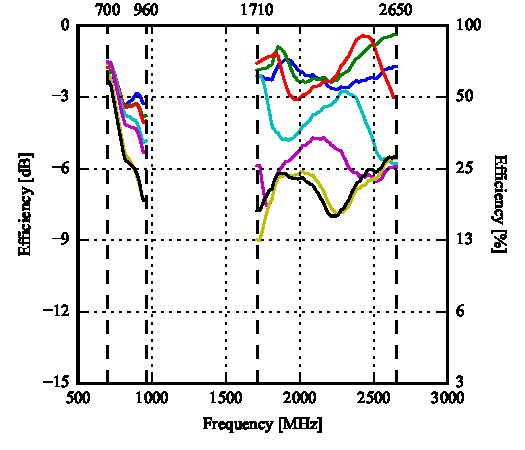
\includegraphics{img/tech_sol/trianglefeed/mockup/sweep_efficiency_top.pdf}
        \caption{Top antenna, sweeping the top antenna and fixing the side antenna.}
    \end{subfigure}
    \hfill
    \begin{subfigure}{0.49\linewidth}
        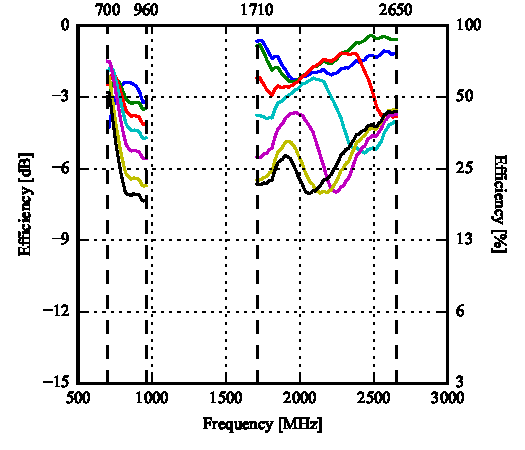
\includegraphics{img/tech_sol/trianglefeed/mockup/sweep_efficiency_side.pdf}
        \caption{Side antenna, sweeping the side antenna and fixing the top antenna.}
    \end{subfigure}
    \caption{Total efficiency for each of the antennas when sweeping the shunt-capacitor values.}
    \label{fig:triang_proto_sweep_efficiency}
\end{figure}
